\appendix

\pagebreak
\section{GitHub Repository README}

The following content is the README file taken from the FANS GitHub repository.

\def\pdffile{../../README.pdf}

\begin{center}
    \includegraphics[width=5in, page=1]{\pdffile}

    \includegraphics[width=5in, page=2]{\pdffile}

    \includegraphics[width=5in, page=3]{\pdffile}

    \includegraphics[width=5in, page=4]{\pdffile}

    \includegraphics[width=5in, page=5]{\pdffile}

    \includegraphics[width=5in, page=6]{\pdffile}

    \includegraphics[width=5in, page=7]{\pdffile}

    \includegraphics[width=5in, page=8]{\pdffile}
\end{center}

\section{Additional Use Cases} \label{ap:sequence}

The following sub-sections describe additional use cases that are handled by FANS, along with their sequence diagrams.

\subsubsection{Add New Contact Information Use Case}

The use case shown in Figure \ref{fig:add-contact} outlines the process of adding new contact information to the FANS
database. Through the web GUI, a user enters a new contact (name, email, phone, etc.) to be subscribed to emergency
notifications. Upon submission, these details are updated in the real-time cloud database. The notification system also
copies these changes to its local database a backup for possible connection loss.

\begin{figure}
    \centering
    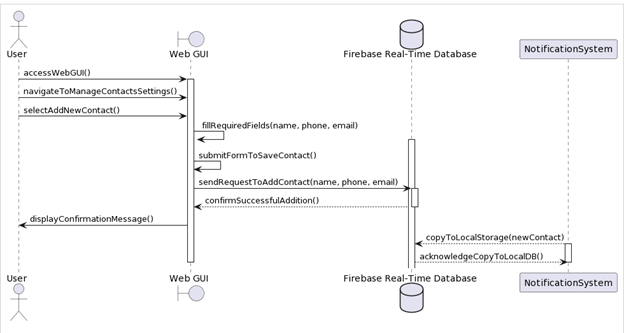
\includegraphics[width=\imagewidth]{../assets/sequence/AddingNewContactInformationSequenceDiagram.png}
    \caption{The sequence diagram for the adding new contact information use case.}
    \label{fig:add-contact}
\end{figure}
